
\chapter{Diseño}

\lettrine{E}{n} este capítulo describiremos la estructura de clases de los dos sistemas realizados en este trabajo.

\section{Análisis de sentimientos}

El sistema de análisis de sentimientos estará compuesto por una superclase Classificator que contendrá métodos y parámetros comunes a las clases Machine Learning y Deep Learning. Estás dos subclases implementarán de forma individual el comportamiento de los métodos de entrenamiento y predicción. Para realizar el preprocesado de los documentos se creará la clase VectorizerHelper que extenderá de las clases de la biblioteca sklearn BaseEstimator y TrasformerMixin, esto nos permitirá utilizar esta clases como parte del pipe de la búsqueda de parámetros.

\subsection{Diagrama de clases}

\begin{figure}[H]
	\centering
	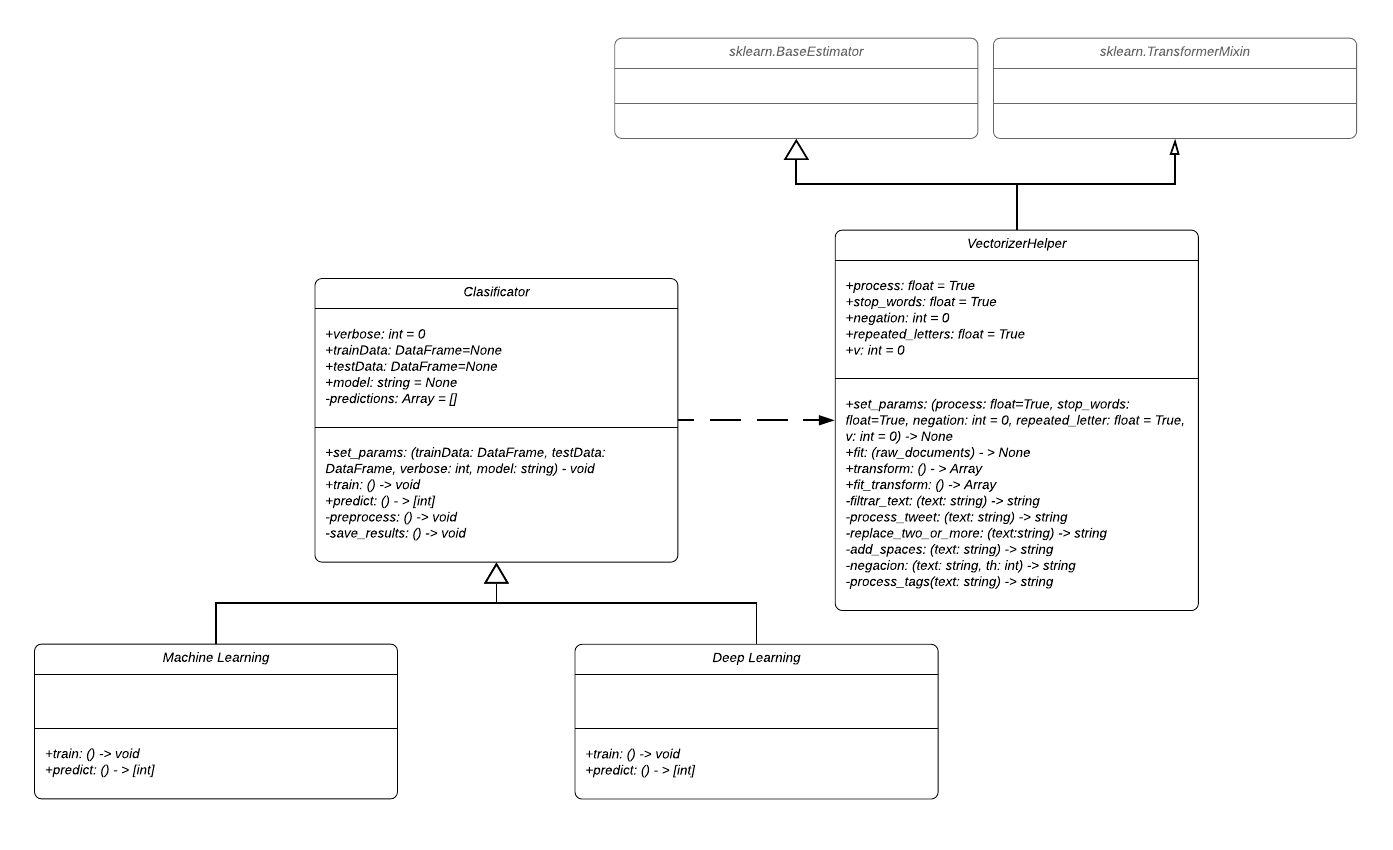
\includegraphics[width=1\textwidth]{imaxes/saClases.png}
	\caption{Diagrama de clases del sistema de análisis de sentimientos}
	\label{saClases}
\end{figure}

\section{Servicio web}

En esta sección se mostrará el diagrama de clases del servicio de comentarios. En la figura \ref{entClases} vemos la relación de las clases entidad relacionadas al comentario. En la figura \ref{daoClases} se describe la estructura del controlador y el servicio de comentarios, así como la descripción del DTO (Data Transfer Object) devuelto por el servicio. 

\subsection{Diagrama de clases}

\begin{figure}[H]
	\centering
	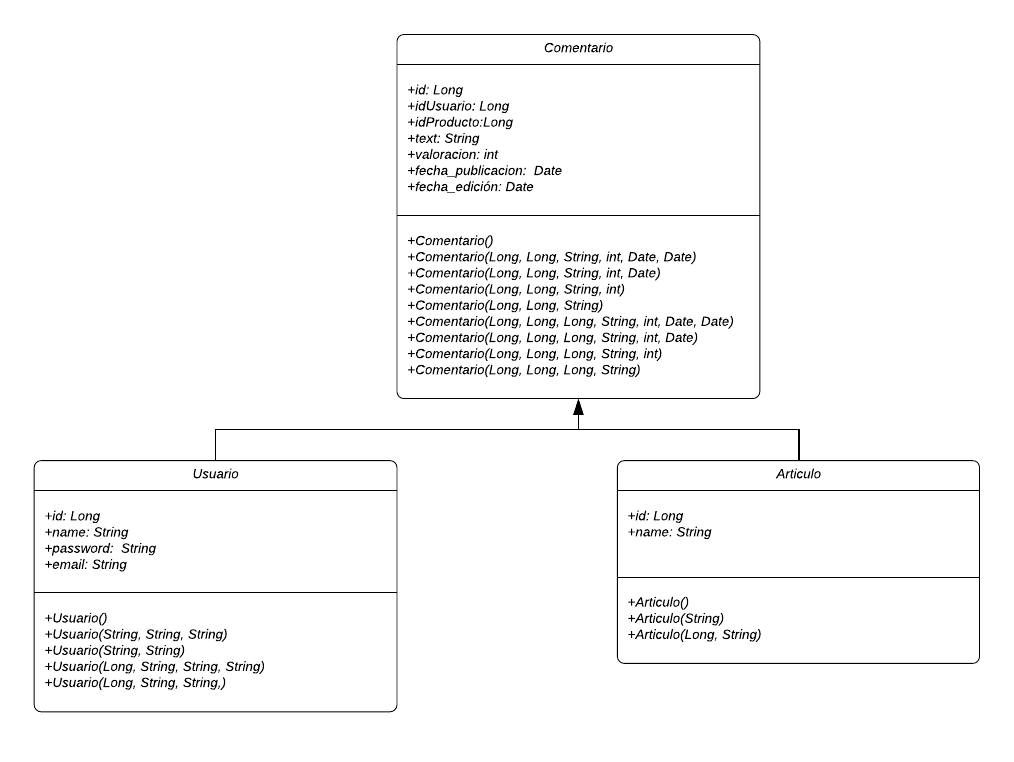
\includegraphics[width=0.75\textwidth]{imaxes/entClases.png}
	\caption{Diagrama de clases de las entidades del modelo SQL}
	\label{entClases}
\end{figure}

\begin{figure}[H]
	\centering
	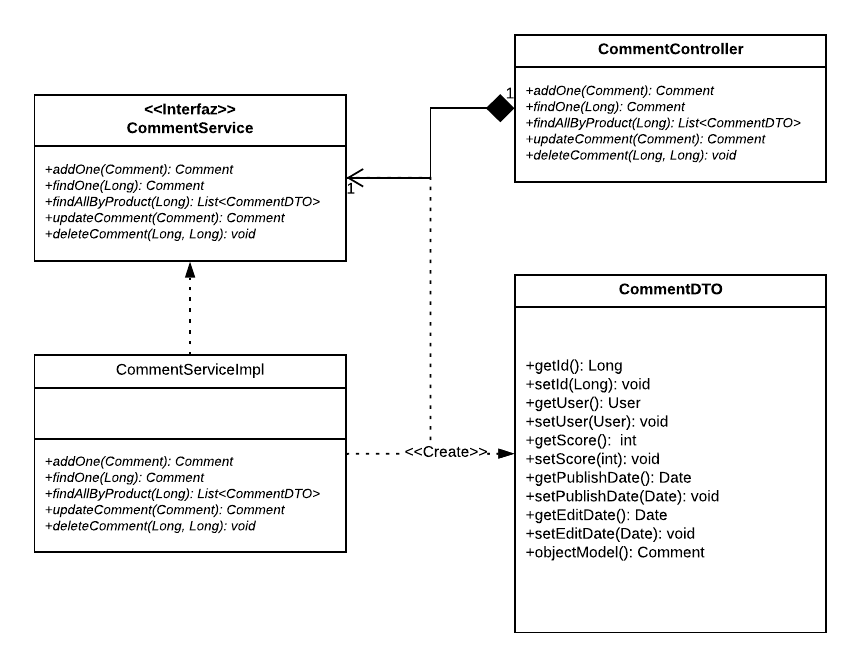
\includegraphics[width=0.70\textwidth]{imaxes/daoClases.png}
	\caption{Diagrama de clases de comentario.}
	\label{daoClases}
\end{figure}